\CHAPTER{The LIGO detector}
\label{chapter2}
\doublespace

\SECTION{Science Runs}
\SECTION{LIGO Scientific Collaboration}
\checkme{CURRENTLY STOLEN FROM MY GEN EXAM DOC!!!}
I assume in this section that the reader has a basic understanding of the LIGO detectors and the effect of gravitational waves on such a detector.  This section will thus
focus on a slightly more detailed description of instrument
noise and data in order to provide context for the rest of
this paper.  We have already seen in \ref{sec:signals} the 
importance of correctly characterizing an instruments noise
and bandwidth.

\SUBSECTION{DATA}

The gravitational wave information is encoded in several channels
which are sampled at 16384Hz with 16 bits of dynamic range.  
This makes the absolute bandwidth of LIGO instruments restricted
to $(0,8192]$ Hz (the Nyquist frequency). 

Unfortunately LIGO GW data is not continous.  Each detector
has a limited duty cycle caused from commissioning downtime and
lock loss from external disturbances.  This means that the
total amount of data in coincidence is reduced.  Additionally
many environmental monitors are used to establish the quality
of data.  For example, we will see in the next section how important 
seismic noise is for LIGO's operation.  For that reason several
seismometers and other instruments record ground motion, other environmental disturbances, and their effect near every test masse in order
to establish times when data may be suspect.  Depending on the
specific search these times may also contribute to a loss in
live time.  

\SUBSECTION{NOISE}
Although LIGO is effectively a broadband detector frequency
dependent noise greatly reduces its sensitivity at very
low and very high frequencies.  Thus it is useful to discuss, in the next few 
sections, briefly the noise sources in LIGO since it's effective bandwitdth is limited by these several sources
and others.  The arguments below come mostly from Saulson \cite{Saulson}.

Before I discuss sources of noise it is useful to set a goal
for the characteristic strain of binary inspirals \cite{300years},
\begin{equation}
h_c = 4.1\times10^{-22}\left({\frac{\mu}{M\odot}}\right)^{1/2}\left({\frac{M}{M\odot}}\right)^{1/3}\left({\frac{100Mpc}{r}}\right)\left({\frac{100Hz}{f_c}}\right)^{1/6}
\end{equation}
where $f_c$ is the characteristic frequency at which the
detector has the lowest strain noise.  
For an optimally oriented neutron star inspiral at the Virgo cluster's distance (15 Mpc) one will
have about $10^{-21}$ strain.  However it is important to have
a broad response around the characteristic frequency $f_c$ since
for matched filtering the SNR will grow with the time that
a signal remains in band.

\SUBSUBSECTION{SEISMIC MOTION}
Seismic noise is by far the largest overall contributor to LIGO 
noise.  The fundamental coupling comes through the suspension
of the test masses.  Since we cannot have mirrors actually free falling (for long) we have to suspend them via wires, which of course act as a pendulum.  The resonant
frequency of the pendulum modes are all approximately $\leq 1Hz$.  This guarantees
large motion at low frequencies where seismic disturbances
dominate thus giving very low sensitivity to GWs.
If you just consider the ideal simple pendulum's response to 
seismic noise the gravitational wave strain sensitivity would
be \cite{Saulson} (assuming ground motion with displacement
noise $x(f) = 10^{-7}cm/\sqrt{Hz}(10Hz/f)^2$ above 10Hz.),
\begin{equation}
\label{SeismicNoise}
h(f) \sim 5 \times 10^{-11}{\left(\frac{1Hz}{f}\right)}^4 /\sqrt{Hz}
\end{equation}
This requires a frequency of nearly $1kHz$ in order to reach
the desired strain of $1\times10^{-21}/\sqrt{Hz}$\cite{Saulson}.  This would exclude several high mass systems
which merge before reaching that frequency.  It also is
not benificial for low mass systems since SNR will grow
with the time that a signal spends in a low noise region.  Clearly
additional seismic isolation is necessary.  This is done in
two ways.  One is passive isolation which empolyes the use
of mass-spring pairs to add additional high frequency 
supression.  The other is active isolation whereby
the motion of the test mass housing is corrected by applying
the appropriate counter motion \cite{HEPI}.  Active seismic
isolation was necessary at the LIGO Livingston Observatory 
due higher than usual low frequency noise as indicated in
figure \ref{f:LLOseism}. 

Simple passive isolation alone adds more frequency poles
to the strain noise each providing a similar supression as
(\ref{SeismicNoise}) (thus making the overal supression much
steeper).  Of course things are further complicated
when considering the vibrational modes of the pendulum
wires themselves which show up in the spectrum as 
higher frequency peaks.  Nevertheless careful passive isolation
reduces the low frequency noise floor to be able to reach
the desired strain noise at $\sim 50Hz$ instead of $1KHz$.

\SUBSUBSECTION{SHOT NOISE}
The discrete arrival of photons at the detector output provides
a limit to LIGO's ability to measure phase changes.  The simple
expression for shot noise is \cite{Saulson}
\begin{equation}
h_{shot} = \frac{1}{L}\sqrt{\frac{\hbar c\lambda}{2\pi P_{in}}}
\end{equation}
Where $P_{in}$  is the input laser power.  Here the noise
has no frequency dependence (it is white) with an amplitude that scales inversely as the square root of the laser power.  
The transfer function of the LIGO's Fabry-Perot cavity actually
gives the shot noise a scaling that goes as $\propto f$. The
next section describes why increasing the laser power to
arbitrarily high values doesn't gaurantee lower noise.

\SUBSUBSECTION{RADIATION PRESSURE}
Light does exert a force on whatever it interacts with.  The
notion of radiation pressure provides a fundamental reason
why you cannot just crank up the laser power in hopes of
reducing your shot noise.  Although it is true that you will
reduce shot noise, the noise created by pressure will soon
dominate.  This noise has (as you would expect) the opposite
scaling with laser power \cite{Saulson} and for a simple Michelson
is,
\begin{equation}
h_{rp} = \frac{1}{mf^2L}\sqrt{\frac{\hbar P_{in}}{2\pi c^3 \lambda}}
\end{equation}

\SUBSUBSECTION{THERMAL NOISE}
The scaling of seismic noise $\propto f^{-n}$ and shot noise
in a Fabry-Perot $\propto f^2$ give the limiting low and high frequency components respectively.  The \emph{in between} is dominated by
thermal noise in the test masses and suspension wires. 
Derivation and accounting for this is probably beyond the
scope of this document.  I have provided a recent noise
spectrum in figure \ref{f:spectrum}.

%\begin{figure}[h!]
%\begin{center}
%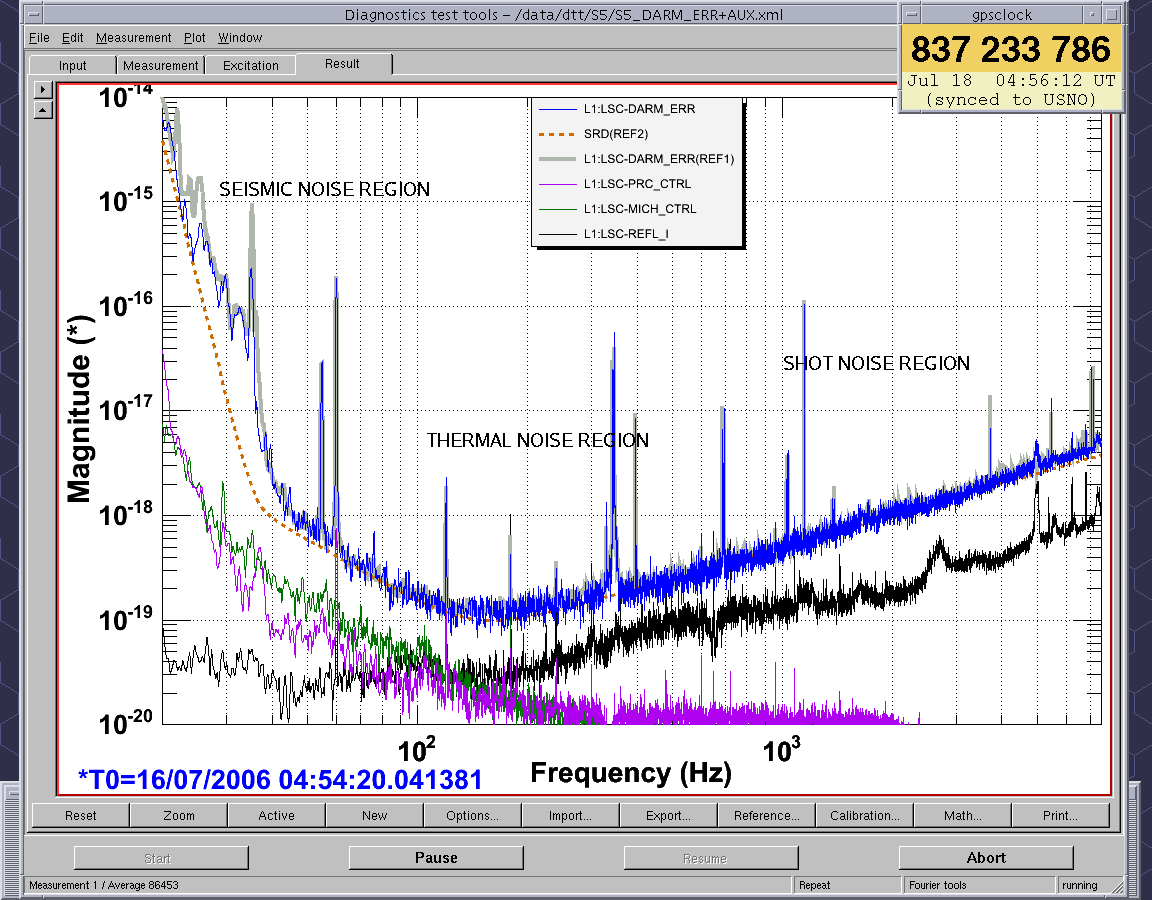
\includegraphics[width=0.7\textwidth]{chapter2/spectrum.png}
%\caption{\label{f:spectrum}LLO noise spectrum}
%\end{center}
%\end{figure} 
%\SECTION{TBD}
%\SUBSECTION{TBD}
